\documentclass{article}
\usepackage[utf8]{inputenc}
\usepackage{amsmath}
\usepackage{amssymb} 
\usepackage{soul}
\usepackage{ulem}
\usepackage{graphicx}
\usepackage{grffile} % allow use .eps files
\usepackage{float}

\title{Kernel Smoothing And Heat Equation}
\date{\today}

\begin{document}

\maketitle

\section{Notes}
\label{sec:notes}

\begin{itemize}
% 12/01/2020  
\item 12/01/2020. 
\begin{figure}[H]
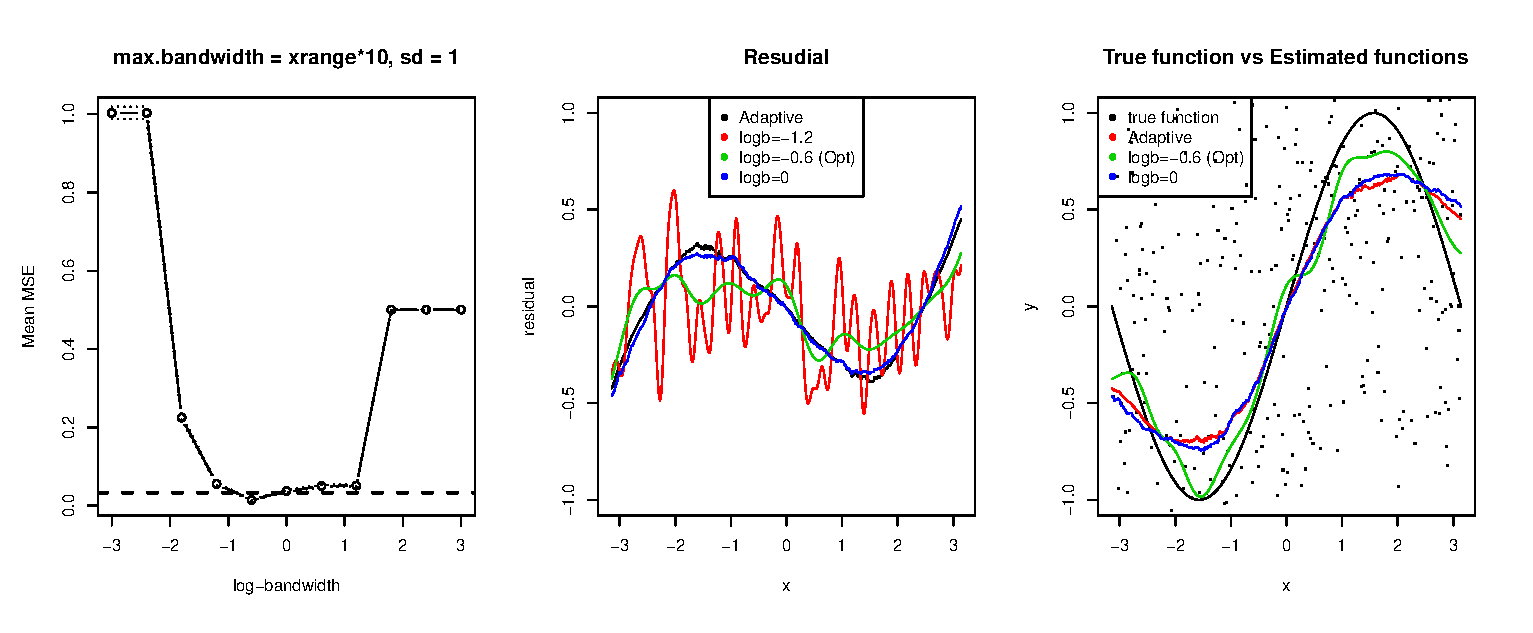
\includegraphics[width=\linewidth]{pic/sim.plot1.eps}
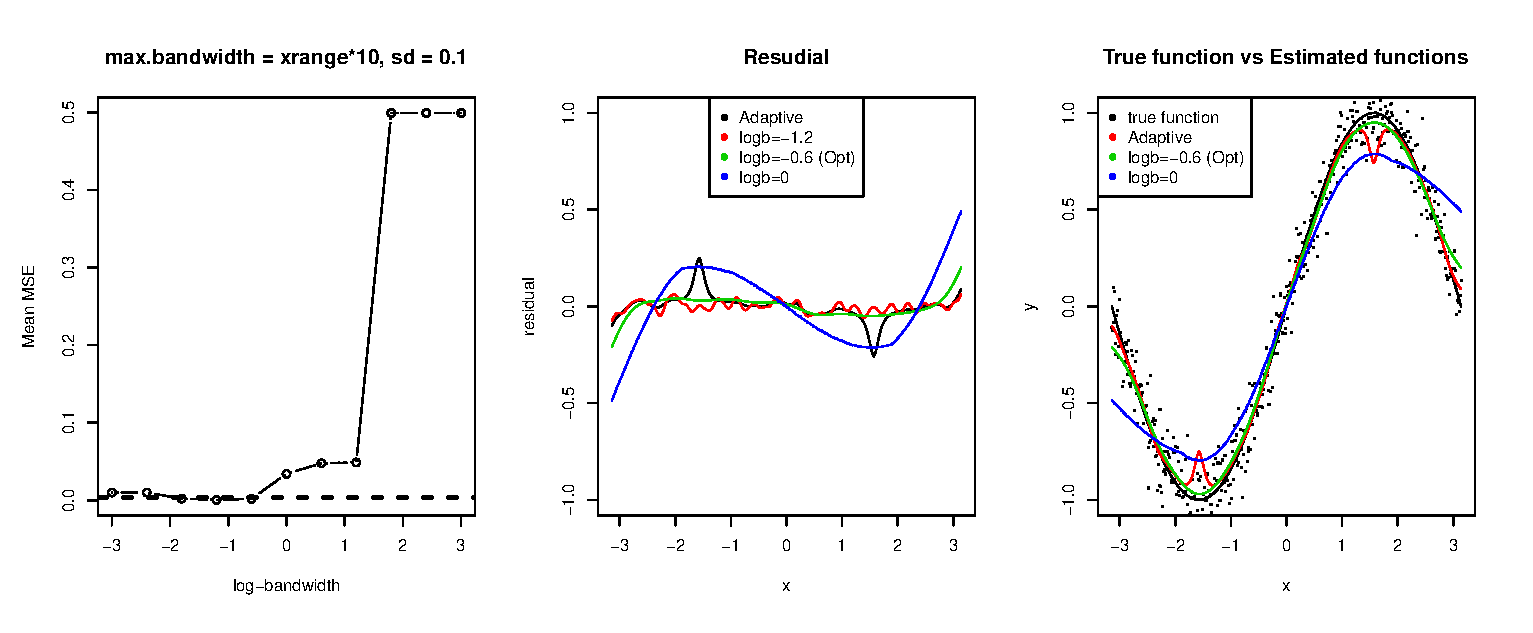
\includegraphics[width=\linewidth]{pic/sim.plot2.eps}
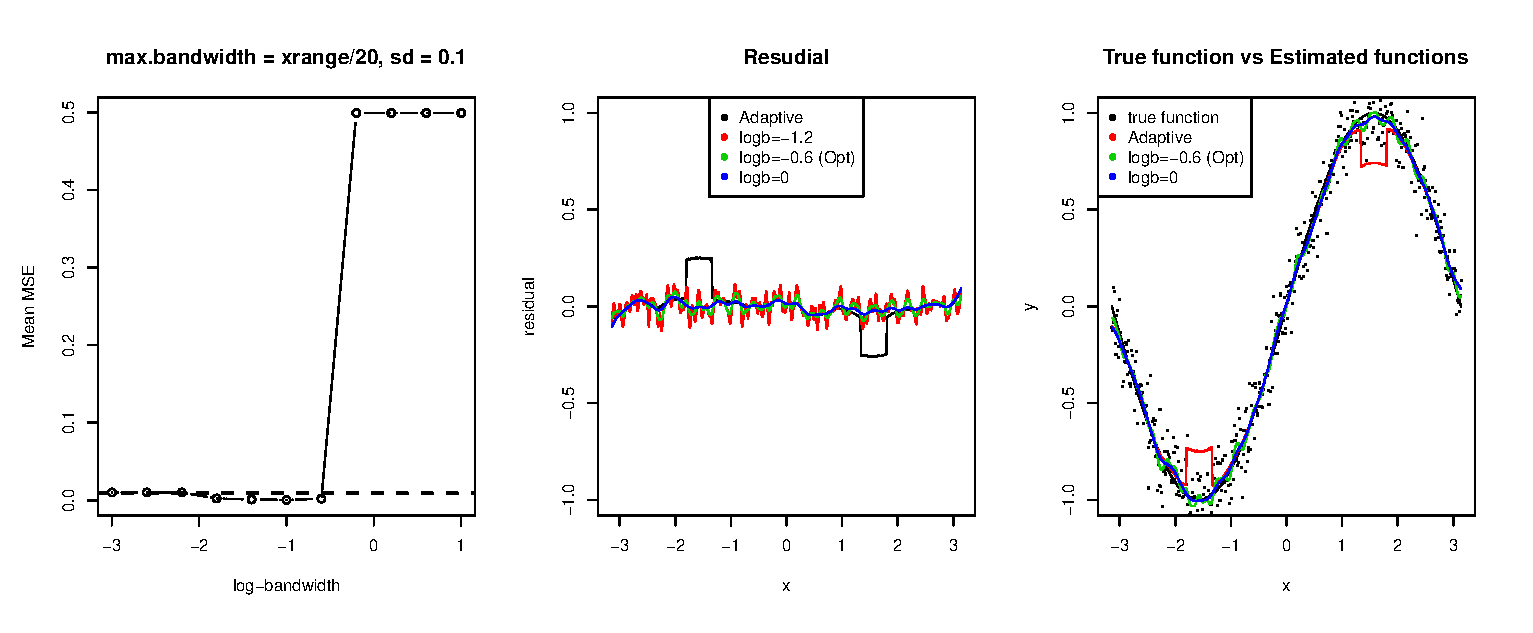
\includegraphics[width=\linewidth]{pic/sim.plot3.eps}
\end{figure}

The boundary behavior of the adaptive scenario is not ideal. We then modified $\texttt{max.window}$ from $\texttt{xrange/5}$ to $\texttt{xrange/0.1}$. The situation gets better. 

We explored the extreme points by 
\begin{enumerate}
\item computing the difference between the empirical value \texttt{mean(y.within.window)} and the true value \texttt{u}
\item comparing the empirical MSE with the theoretical MSE of the extreme points
\end{enumerate}

Denote $\texttt{max.window} = \frac{\texttt{xrange}}{k}$, we plot the difference between the empirical value \texttt{mean(y.within.window)} and the true value \texttt{u} with respect to $k$ at extreme points. We noticed when $k>2$, the difference would increase tremendously (Figure below).

\begin{figure}[H]
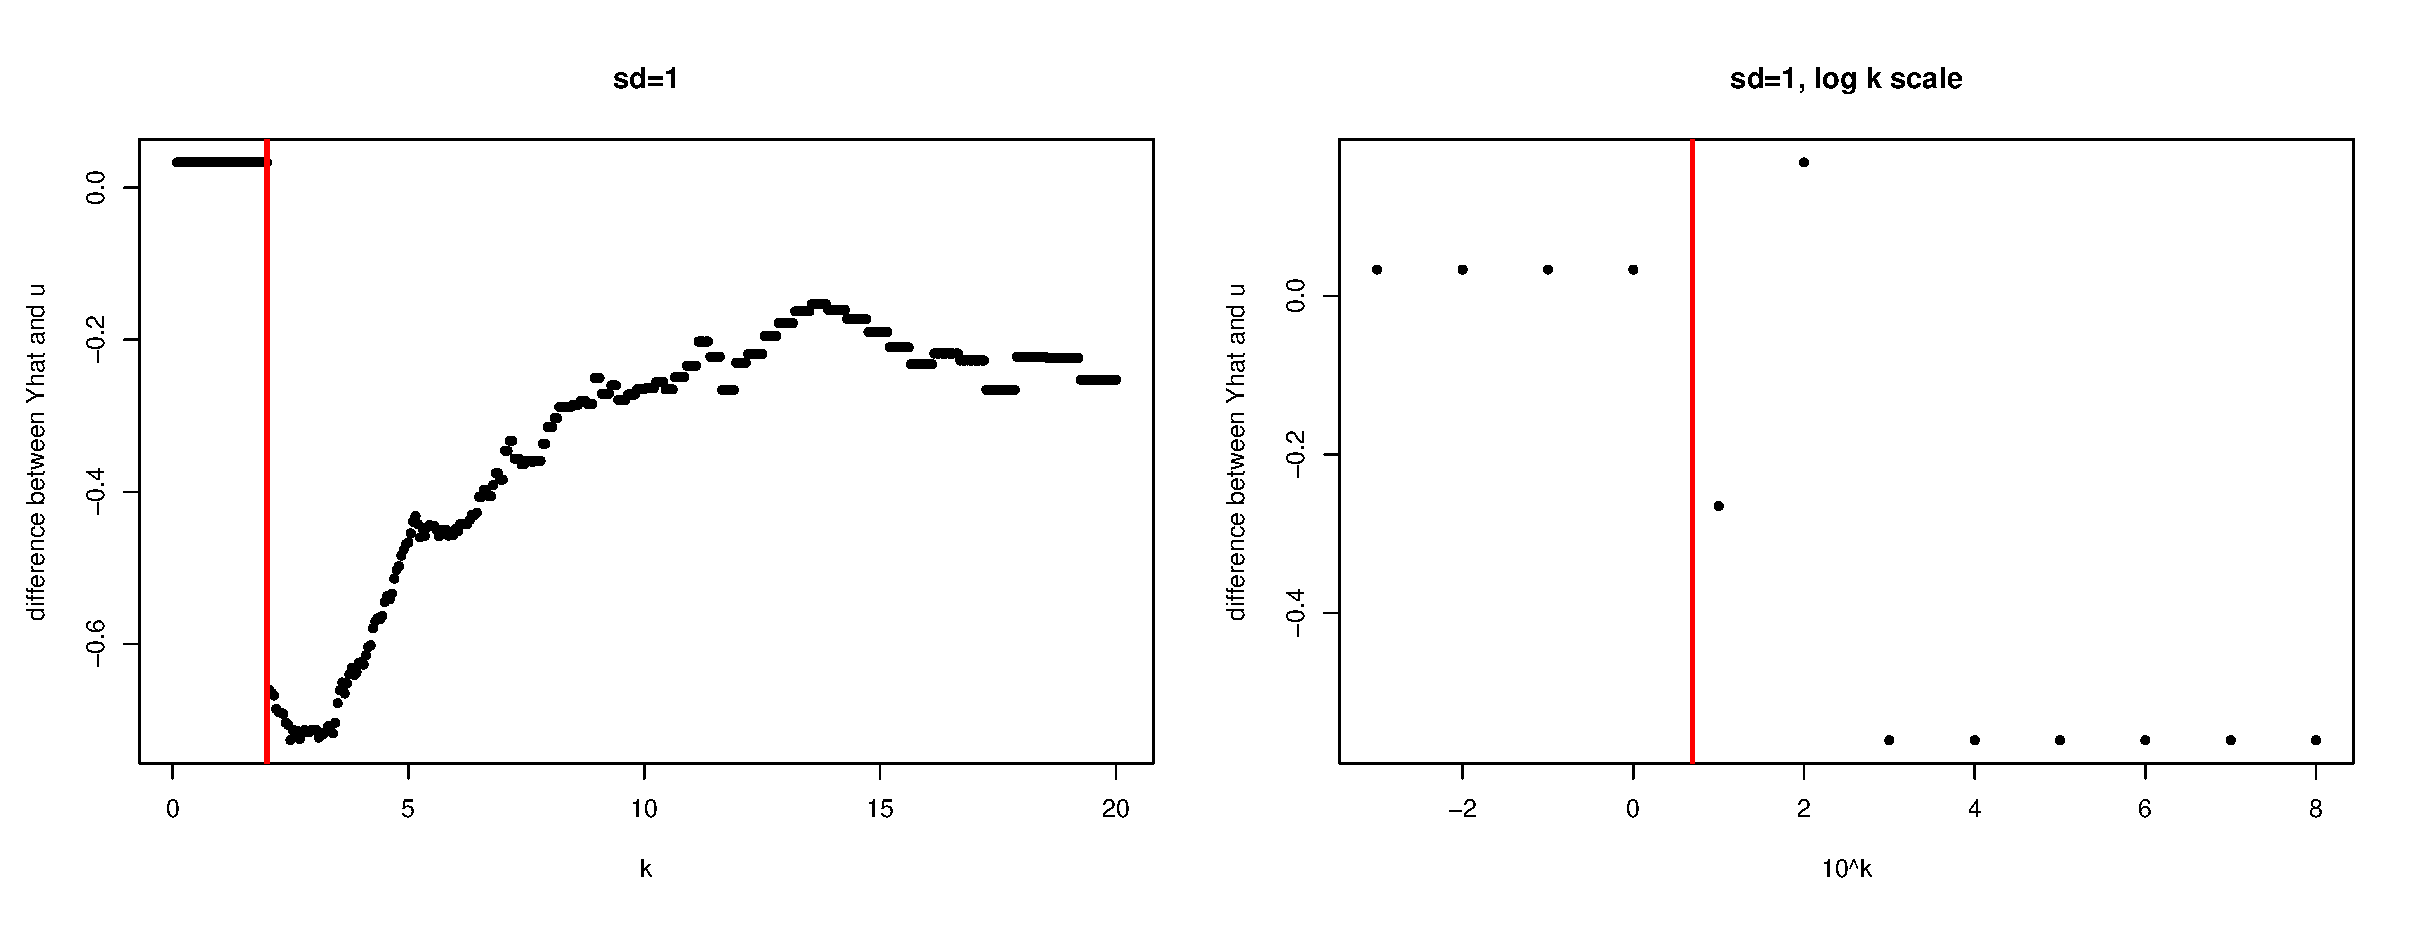
\includegraphics[width=\linewidth]{pic/sim.plot4.eps}
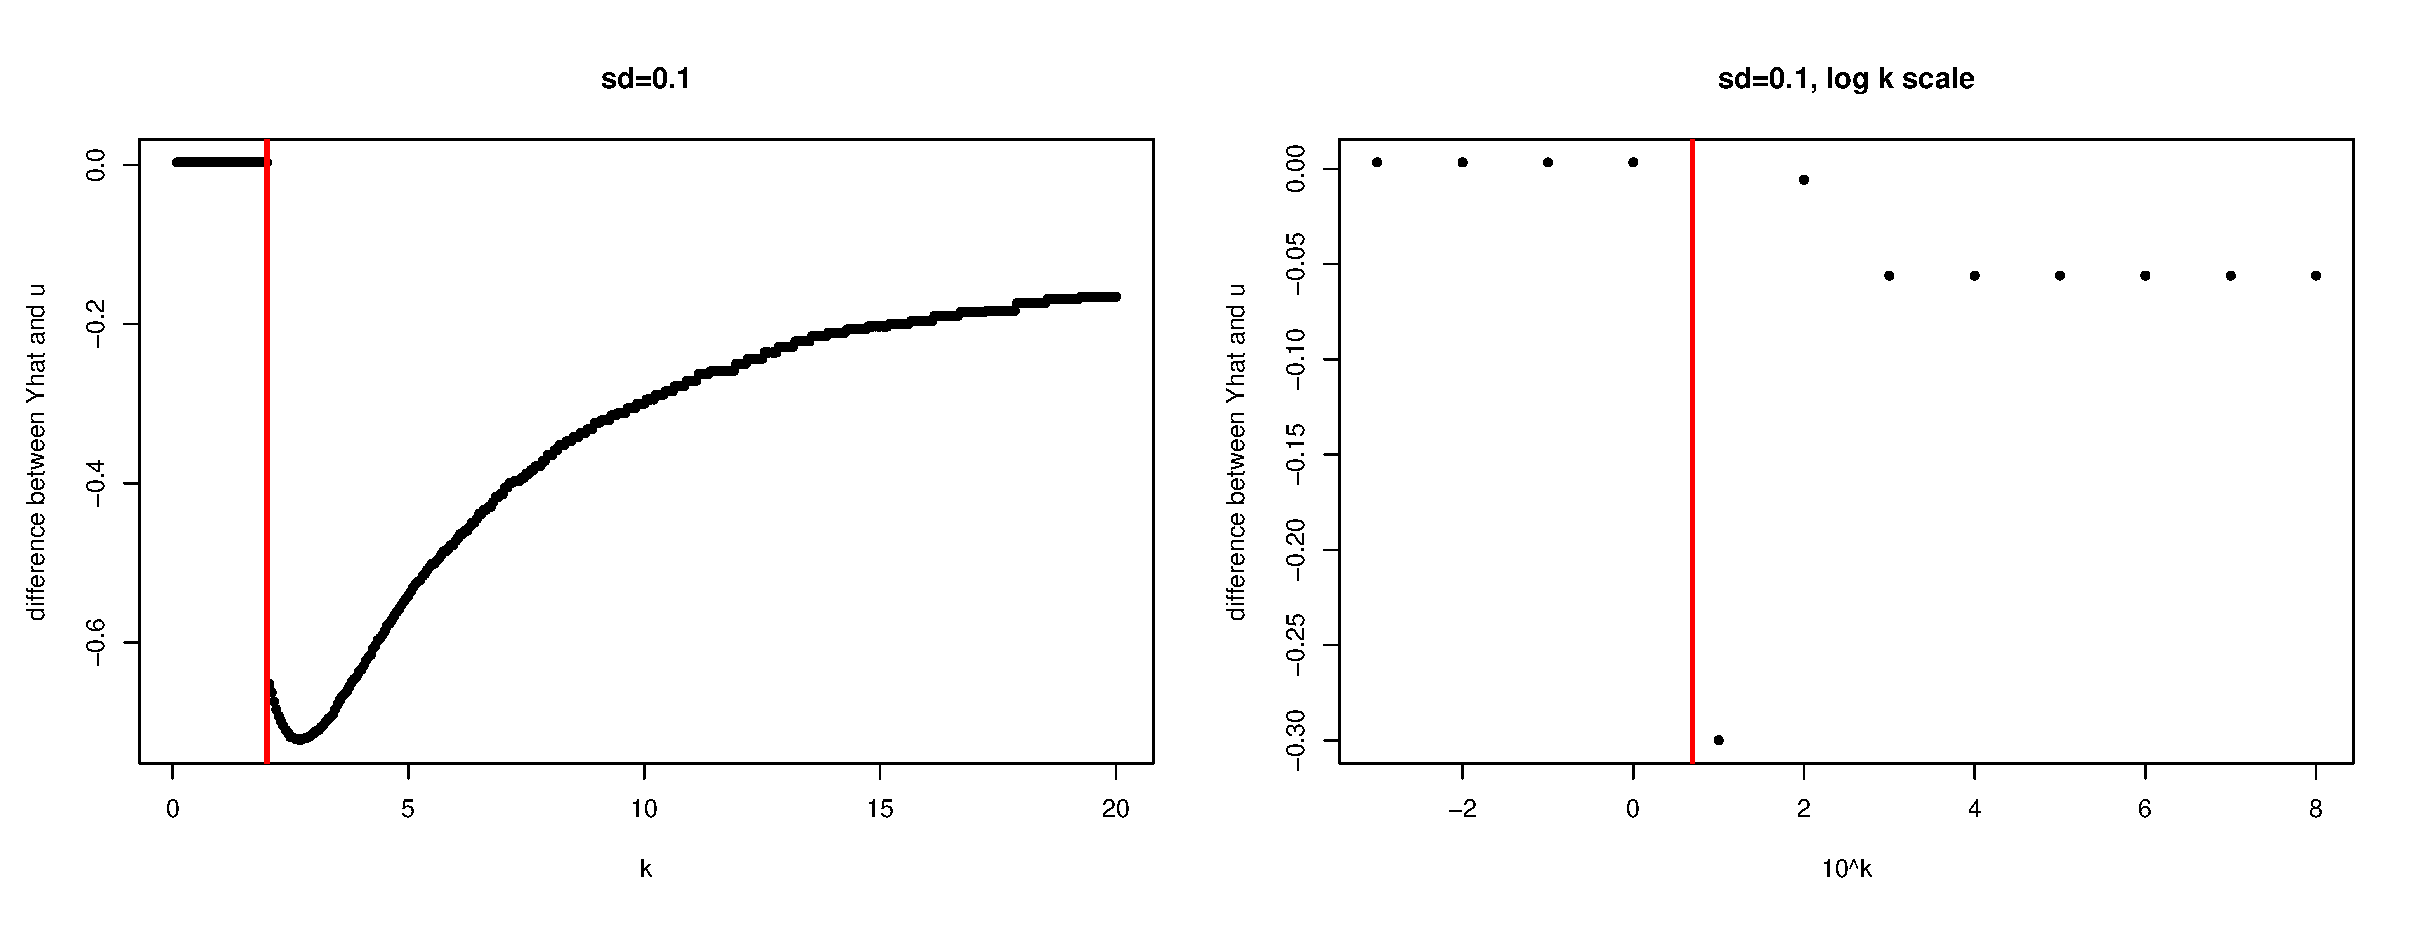
\includegraphics[width=\linewidth]{pic/sim.plot5.eps}
\caption{Extreme point (first point) of $y=\sin(x)$ with $\sigma = 1$ and  $\sigma = 0.1$ scenarios. We use log-scale plot to see if the difference would converge asymptomatically as $k\rightarrow +\infty$. The red line denotes when $k=2$, the difference has a jump.} 
\end{figure}


% 11/17/2020  
\item 11/17/2020. 

TODOLIST:
\begin{enumerate}
\item Editor: Emacs, Vim
\item Learn: Command line, \texttt{ssh}, \texttt{zsh},\texttt{bash}, to remotely control.
\item \texttt{.eps} $\rightarrow$ \texttt{.eps}; change \texttt{postscript()} to \texttt{pdf(), png(), tiff()}
\item Residual trend means under-smoothing (overfitting)
\item manually compute the 2 extreme points (second order taylor expansion) -- empirical MSE and theoretical MSE
\end{enumerate}

% 11/10/2020  
\item 11/10/2020. We implemented circular smoother on both fixed bandwidth and adaptive bandwidth scenarios; and did the corresponding simulation. We noticed for the circular data, the adaptive bandwidth cannot beat the optimal fixed bandwidth. Fixed bandwidth achieve the smallest MSE in our $y=\sin(x)$ setting. We also noticed the circular smoother performs better than Euclidean smoother in the circular data ($y=\sin(x)$). 

\begin{verbatim}
           euclidean   circular
Adaptive  0.19821445 0.19821445
logb=-3   1.00313133 1.00313133
logb=-2.4 1.00313133 1.00313133
logb=-1.8 1.00313133 1.00313133
logb=-1.2 0.11346202 0.11227971
logb=-0.6 0.02875581 0.02717735
logb=0    0.08004308 0.08145240
logb=0.6  0.44585526 0.52684029
logb=1.2  0.49326980 0.50454607
logb=1.8  0.50018979 0.50094139
logb=2.4  0.50068896 0.50068896
logb=3    0.50068896 0.50068896
\end{verbatim}


TODOLIST:
  \begin{enumerate}
    \item Compare MSE at 2 boundaries 
    \item manually do the smoothing for certain points, compare the two bandwidth (adaptive vs fixed); expected MSE and empirical MSE should agree. Two scenarios:
    \begin{enumerate}
    \item manual result doesn't equal to the automatic one, debug the result
    \item manual result equal to the auto one. Seek the reason: Taylor expansion is not good enough, higher order term is needed (More observation, smaller bandwidth, smaller window)
    \end{enumerate}
    \item Future: explore the inhomogeneous heat equation (adaptive $\lambda(x)$) 
    $$\frac{\partial f(x,t)}{\partial t}  = \Delta f = \frac{\partial f}{\partial x}[\lambda(x)\frac{\partial f}{\partial x}] \neq  \lambda(x)\frac{\partial^2 f}{
    \partial x^2} $$

    Google the connection between adaptive smoothing and inhomogeneous heat equation 
  \end{enumerate} 



% 10/27/2020  
\item 10/27/2020. We reviewed Dr. Qiu's code/documentation. Todos:
  \begin{enumerate}
  \item Compare our old code with Dr. Qiu's new code one more time.
  \item Try to implement the circular smoother (at least for the fixed bandwidth case).
  \item We've already studied the mathematical connections between the classical (homogeneous) heat equation and Gaussian kernel smoothing. We need to document this important connection in this document.
  \item We need to think: what is the mathematical connection between \emph{adaptive Gaussian kernel smoother} and \emph{inhomogeneous} heat equation?  Rationale: we've already derived (based on large sample theory) the ``optimal'' variable bandwidth for kernel smoother. If the kernel smoother is equivalent to an inhomogeneous differential equation, it means that we can then use an efficient numerical DE solver (e.g., those based on finite element method) to do kernel smoothing, especially for multi-dimensional cases.
  \item In the long run, we need to develop a practical estimation procedure for $x(t)$ and $\sigma^{2}(t)$, better with some model selection procedure so the entire estimation procedure can be automated.
  \item Multi-dimensional!! (a) the curse of dimensionality, (b) much more complicated boundary to deal with.
  \end{enumerate}
\end{itemize}


\section{Introduction}
 
It is universally acknowledged that observed data with respect to the underlying patterns we are seeking for in the physical world is, to some extent, contaminated with random noise. Commonly, the observed data would be expressed into two parts: the systematic component (i.e.: a true underlying oracle function $u(x)$) and a random component (i.e.: noise $\epsilon$). Yet, due to the fundamental sorrow of the limited observations in an infinite world, we may fail to achieve the oracle function. In fact, we can only estimate it based on our finite noise infested observations. 

For decades, statisticians have been proposed various methods to estimate the oracle function. One of the non-parametric ways is to use direct diffusion to smooth away all the noise. In an absolute non-rigorous sense, the direction diffusion process achieves the oracle risk by (weighted) averaging each observation neighbor. Each time we do this, our estimated function will be closer to the true function until at a finite time $T$ we achieve our goal. After that the estimated function will be bounded away from the truth. People coin the term "over-smoothing" to indicate this phenomenon. Our goal is to discover the optimal T where we are closest to the truth given an observed data set. 

However, the diffusion process is not widely used among statisticians. Instead, they use kernel smoothing, a nonparametric method proved to be equivalent to the heat equation in physics world. Therefore, finding optimal time T can be translated to the problem of finding the optimal sigma. 
In statistics literature (\ref{} reference needed), the optimal sigma is found to be a constant for every point x. This is a significant constraint. Hence, in this paper, we will allow the spatial bandwidth to be different for each point. In the next section, we will derive the optimal sigma for each observation point. We will do simulations to show that our "adaptive" bandwidth performs better than the best-fixed bandwidth. 


Some literature review...

Goal of this paper...

Structure of the paper...

\section{Methodology}
The connection between Heat Equation and Kernel Smoothing can be expressed (\ref{}reference for Equation (\ref{eq:1})) as
\begin{equation}
    T = \frac{1}{2} \sigma^2         \label{eq:1}
\end{equation} 
where $T$ denotes the total smoothing time in the direction process, and $\sigma$ denotes the proportion of the spatial width of the Gaussian smoother in paper \ref{} (Equation (\ref{eq:2})).
\begin{equation}
    \sigma = \text{bandwidth}\times 0.3706506  \label{eq:2}
\end{equation}
Given $\mathbf{x}_i =(x_1, x_2,...,x_p)^\top \subseteq \mathbb{R}^p $, $Y_i\subseteq R$, we have the data set $$\mathcal{D}_n = \big\{(x_1, y_1),... (x_n, y_n)\big\}$$
Denote $u(\mathbf{x})$ as the oracle function, and $u(\mathbf{x}_i)$ is the first order Taylor expansion
\begin{equation}
      u(\mathbf{x}_i) \approx u(\mathbf{x}) + \frac{\partial u}{\partial \mathbf{x}}(\mathbf{x}_i - \mathbf{x}) 
\end{equation}
And given a Gaussian kernel with $b$ as the bandwidth parameter
\begin{align}
    \phi_b (x) = \frac{1}{\sqrt{2 \pi b}}\exp(\frac{-x^2}{2b})
\end{align}
We have MSE at $\mathbf{x}_i$ with respect to $b$
\begin{equation}
         \text{MSE}_j=  \frac{\sigma^2}{2\sqrt{\pi \cdot b}}  + \left[\frac{\partial^2 u}{2\partial x^2}\cdot b \right]^2
\end{equation}
Take the derivative with respective to $b$, we can solve the equation 
\begin{equation}
    b =\left(\frac{\sigma^2}{2\sqrt{\pi} u''^2}\right)^{\frac{2}{5}} 
\end{equation}
(Detailed calculation in Appendix) 






%-------------- Draft --------------%






\pagebreak

\section{Appendix}


We let

\begin{align*}
    \phi_b (x) = \frac{1}{\sqrt{2 \pi b}}\exp(\frac{-x^2}{2b})
\end{align*}

where b is the band width parameter. Then we have our MSE at $x_i$


\begin{align*}
        \left(\hat{u}(x_i) - u(x_i)\right)  &=  \sigma^2\sum_{i=1}^n  w_i^2  + \left[ \frac{\partial u}{\partial x}\cdot \sum_{i=1}^n  w_i(x_i - x) \right] +  \left[ \frac{\partial^2 u}{2\partial x^2}\cdot \sum_{i=1}^n  w_i(x_i - x)^2 \right] + \sum_{i=1}^n \epsilon_i w_i \\
        E\left[ \left(\hat{u}(x_i) - u(x_i)\right)^2 \right] &= Var\left[ \left(\hat{u}(x_i) - u(x_i)\right) \right] + (E\left[ \left(\hat{u}(x_i) - u(x_i)\right) \right])^2 \\ &=\sigma^2\sum_{i=1}^n  w_i^2  + \left[\frac{\partial u}{\partial x}\cdot \sum_{i=1}^n  w_i(x_i - x)  +   \frac{\partial^2 u}{2\partial x^2}\cdot \sum_{i=1}^n  w_i(x_i - x)^2 \right]^2 \\
   MSE_j =  \sigma^2\sum_{i=1}^n  \phi_b^2(x_j-y_i) & +  \left[ \frac{\partial u}{\partial x}\cdot \sum_{i=1}^n  \phi_b(x_j-y_i)\cdot(x_j - y_i) + \frac{\partial^2 u}{2\partial x^2}\cdot \sum_{i=1}^n  \phi_b(x_j-y_i)\cdot(x_j - y_i)^2 \right]^2
\end{align*}

Now we replace summation with integration

\begin{align*}
     MSE_j &=  \sigma^2 \int_\omega  \phi_b^2(x_i-y)dy  +  \left[ \frac{\partial u}{\partial x}\cdot \int_\omega  \phi_b(x_j-y)\cdot(x_j - y)dy + \frac{\partial^2 u}{2\partial x^2}\cdot \int_{\omega}  \phi_b(x_j-y)\cdot(x_j - y)^2 dy\right]^2\\
     &= \frac{\sigma^2}{2\sqrt{\pi \cdot b}}   + 0 + \left[ \frac{\partial^2 u}{2\partial x^2}\cdot \int_{\omega}  \phi_b(x_j-y)\cdot(x^2_j -2x_j\cdot y + y^2) dy\right]^2\\
     &=  \frac{\sigma^2}{2\sqrt{\pi \cdot b}}   + \left[ \frac{\partial^2 u}{2\partial x^2}\cdot \int_{\omega}  \phi_b(x_j-y)(x^2_j)dy - 2 \int_{\omega}  \phi_b(x_j-y)\cdot (x_j\cdot y)dy +  \int_{\omega}  \phi_b(x_j-y)\cdot y^2 dy\right]^2\\
     &=  \frac{\sigma^2}{2\sqrt{\pi \cdot b}}   + \left[\frac{\partial^2 u}{2\partial x^2}\cdot (x^2_j - 2x^2_j + b + x^2_j) \right]^2\\
     &=  \frac{\sigma^2}{2\sqrt{\pi \cdot b}}  + \left[\frac{\partial^2 u}{2\partial x^2}\cdot b \right]^2
\end{align*}



Set $h(b) = \frac{\sigma^2}{2\sqrt{\pi}}\cdot \frac{1}{\sqrt{b}}+   \frac{1}{4}   u''^2\cdot b^2$, and take derivative, then set $h'(b) = 0$
\begin{align*}
    h'(b)&= -\frac{\sigma^2}{4\sqrt{\pi}}\cdot b^{-\frac{3}{2}}+\frac{1}{2} u''^\cdot b = 0\\
    b &=\left(\frac{\sigma^2}{2\sqrt{\pi} u''^2}\right)^{\frac{2}{5}} 
\end{align*}


















\end{document}
